\documentclass{article}
\usepackage[LGR,T1]{fontenc}
\usepackage[utf8]{inputenc}
\usepackage[greek, english]{babel}
\usepackage{alphabeta}
\usepackage{natbib}
\usepackage{graphicx}
\usepackage{biblatex}
\addbibresource{references.bib}

\def\code#1{\texttt{#1}}

\usepackage{eso-pic}% http://ctan.org/pkg/eso-pic
\usepackage{lipsum}% http://ctan.org/pkg/lipsum

\title{Robustness Diagrams - v0.1}

\author{\\

\includegraphics[width=3in]{safeguard}\\[1ex]\\\\
}

\begin{document}

\maketitle

\newpage

\noident Editor: Θεόδωρος Ντάκουρης - ntakouris@ceid.upatras.gr - 1054332\\
\\

\begin{tabular}{|l|c|c|}
\hline
Όνοματεπώνυμο & email & Αριθμός μητρώου  \\
\hline
Θεόδωρος Ντάκουρης & ntakouris@ceid.upatras.gr & 1054332 \\
Βασίλειος Βασιλόπουλος & vvasil@ceid.upatras.gr &  1054410 \\
Νικόλαος Σουλτάνης & soultanis@ceid.upatras.gr & 1054319  \\
Βάιος Λασκαρέλιας & laskarelias@ceid.upatras.gr & 1054432 \\
Αντόν Παπά & papa@ceid.upatras.gr & 1054337 \\
\hline
\end{tabular}

\renewcommand{\contentsname}{Περιεχόμενα}
\tableofcontents

\section{Διαγράμματα}
Για δική σας ευκολία παρακαλώ να δείτε πέρα από τα screenshots το παρακάτω view-only link από draw.io:

\url{https://drive.google.com/file/d/1AdY8-0ATU-QJPdQeqOm991Y0flZv_5bP/view?usp=sharing}

\subsection{Check In-Out}

\noindent Σημείωση: Παρουσιάζονται και οι 2 περιπτώσεις "μαζί". Τις συγχωνεύουμε για λόγους επαναχρησιμοποίησης και ευαναγνωσίας-ευκολίας. Στην εναλλακτική περίπτωση, ο λόγος αποτυχίας - reason μεταβιβάζεται από controller σε controller μέχρι να φτάσει σε boundary object.

\noindent Check In-Out: \\
\noindent\makebox[\textwidth]{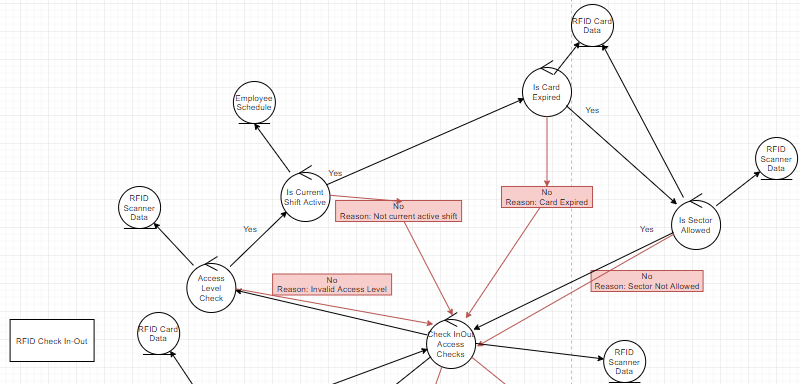
\includegraphics[width=\paperwidth]{robustness1.png}}
\noindent\makebox[\textwidth]{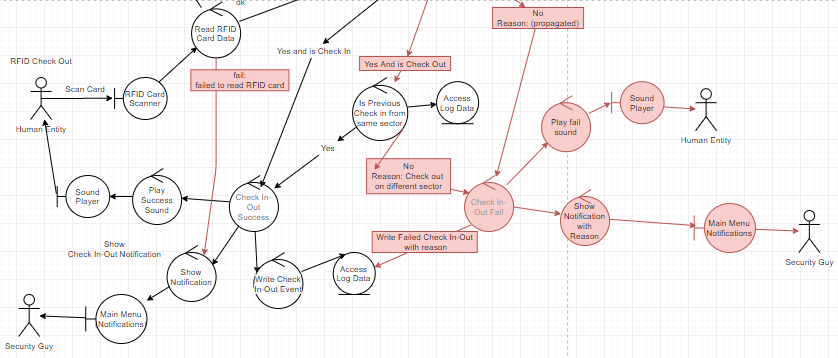
\includegraphics[width=\paperwidth]{robustness2.png}}

\subsection{Insert Employee}
\noindent\makebox[\textwidth]{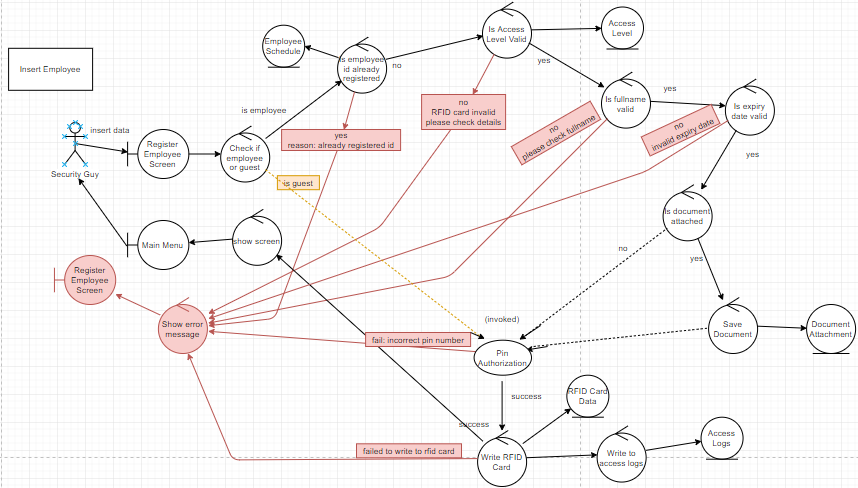
\includegraphics[width=\paperwidth]{robustness3.png}}

\subsection{Delete Employee}
\noindent\makebox[\textwidth]{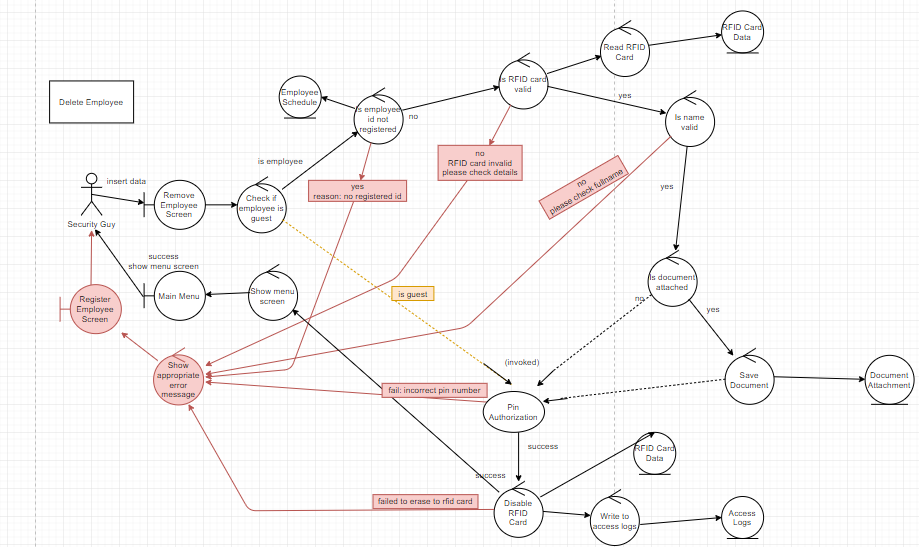
\includegraphics[width=\paperwidth]{robustness4.png}}

\subsection{Browse Access Logs}
\noindent\makebox[\textwidth]{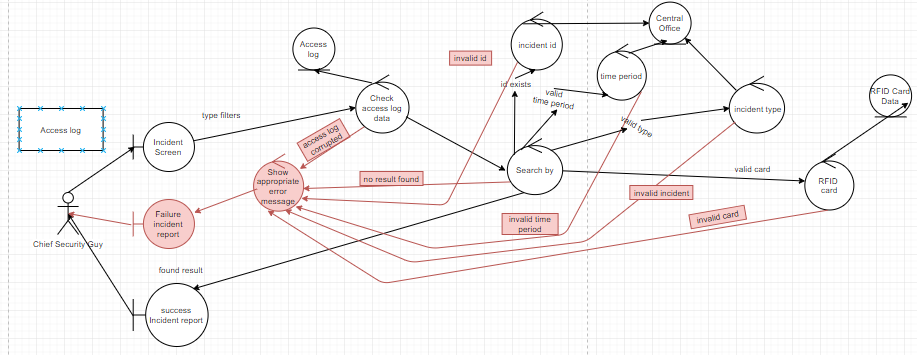
\includegraphics[width=\paperwidth]{robustness5.png}}

\subsection{Drone Notifications}
\noindent\makebox[\textwidth]{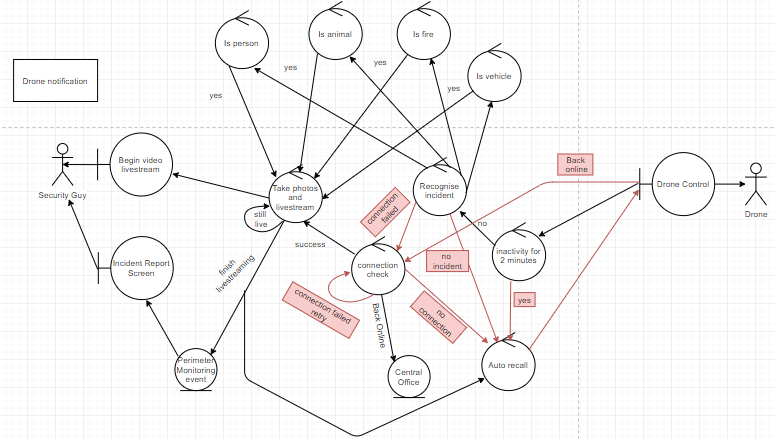
\includegraphics[width=\paperwidth]{robustness6.png}}

\subsection{Incident Submission}
\noindent\makebox[\textwidth]{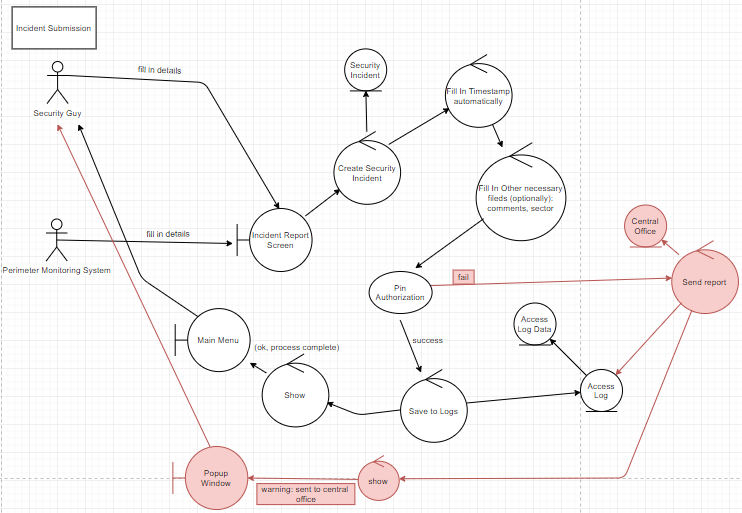
\includegraphics[width=\paperwidth]{robustness7.png}}


\subsection{Send Drone}
\noindent\makebox[\textwidth]{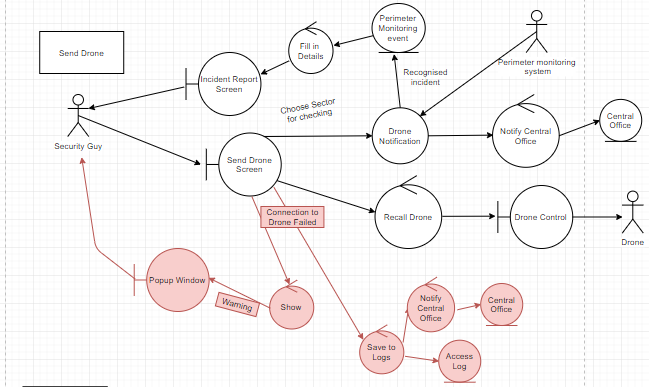
\includegraphics[width=\paperwidth]{robustness8.png}}

\subsection{Silent Alarm}
\noindent\makebox[\textwidth]{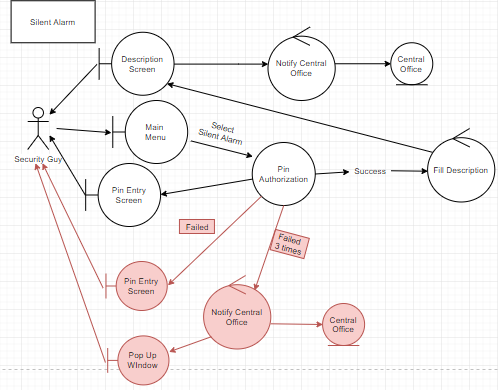
\includegraphics[width=\paperwidth]{robustness9.png}}


\subsection{Pin Authorization}
\noindent\makebox[\textwidth]{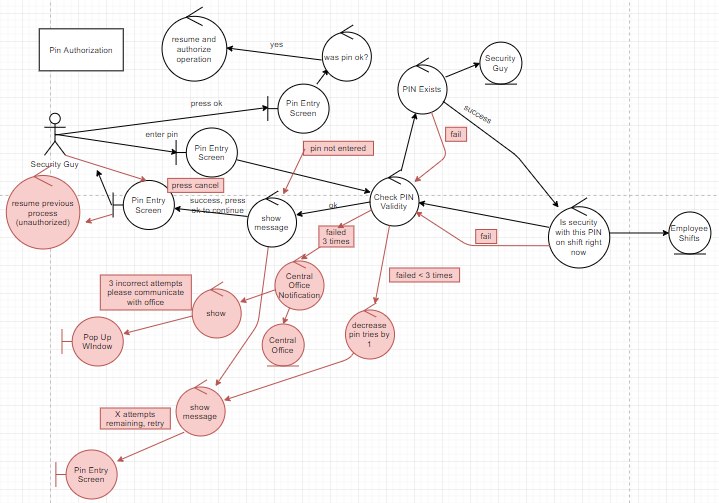
\includegraphics[width=\paperwidth]{robustness10.png}}


\section{Εργαλεία}
Χρησιμοποιήθηκαν:
\begin{itemize}
    \item \LaTeX/Overleaf.com - Συγγραφή του παρόντος τεχνικού κειμένου
    \item Photoshop - Φωτογραφία Σελίδας Τίτλου
    \item draw.io - Σχεδιασμός διαγραμμάτων
\end{itemize}

\end{document}
